\documentclass{standalone}

\usepackage{tikz}
\usetikzlibrary{backgrounds,calc,positioning,decorations.markings}

\begin{document}

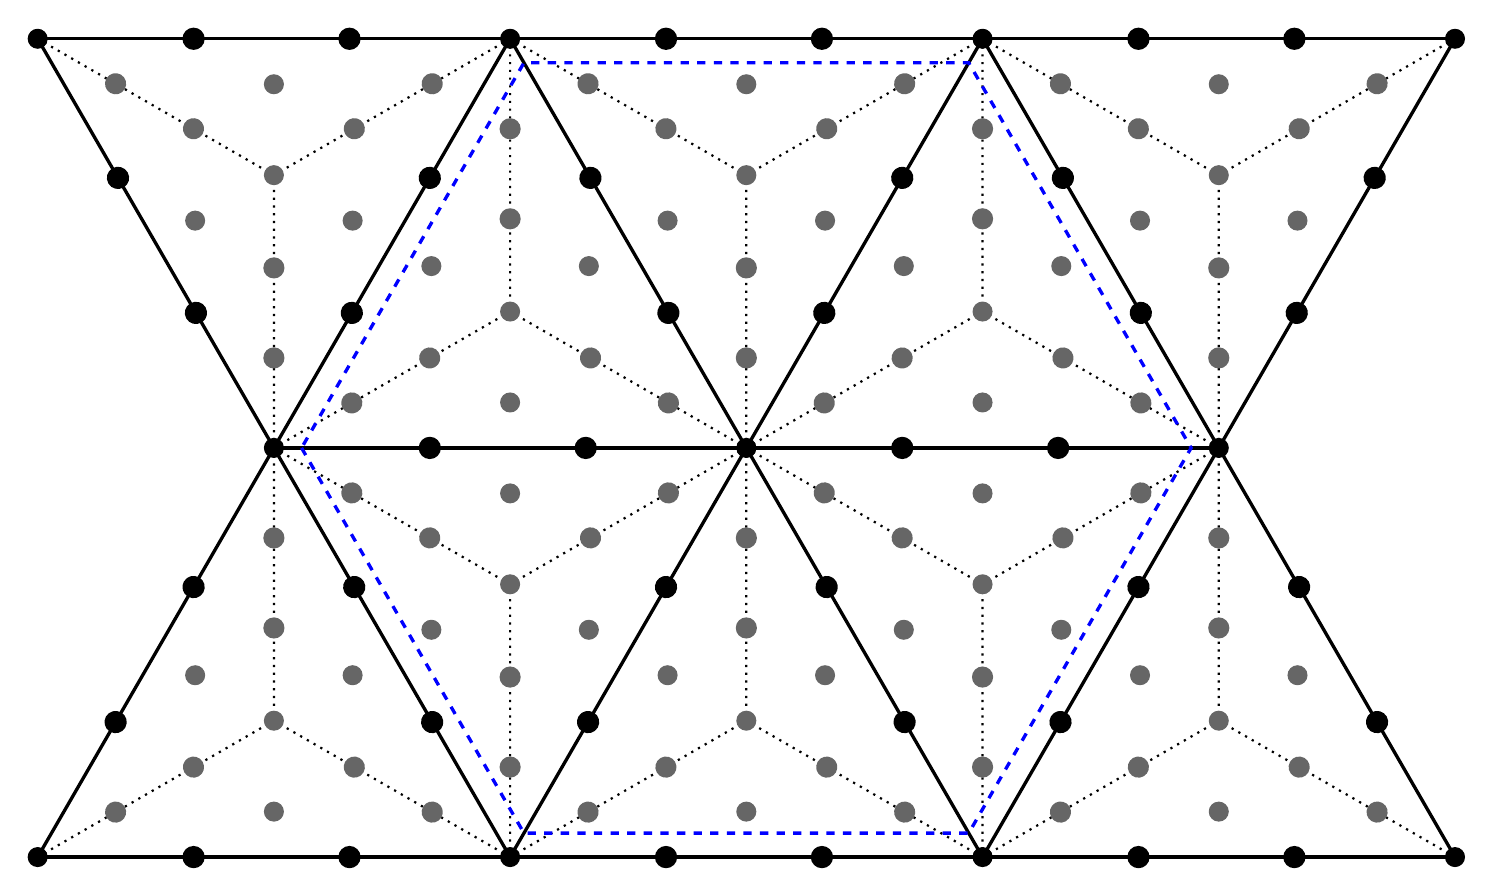
\begin{tikzpicture}[scale=4,
  bcdof/.style={postaction={decorate,decoration={markings,
        mark=between positions 0.33 and 0.66 step 0.33 with {\draw[solid, fill, black!60] circle
          (0.12);}}}},
  dof/.style={postaction={decorate,decoration={markings,
        mark=between positions 0.33 and 0.66 step 0.33 with {\draw[solid, fill, black] circle (0.12);}}}
  }]

  \foreach \i in {0, 1, 2, 3} {
    \coordinate (0-\i) at ($(\i*1.5, 0)$);
    \coordinate (1-\i) at ($(0-\i) + (60:1.5)$);
    \coordinate (2-\i) at ($(1-\i) + (120:1.5)$);

    \foreach \j in {0, 2} {
      \draw[fill] (\j-\i) circle (0.03);
    }
  }
  \foreach \i in {0, 1, 2} {
    \draw[fill] (1-\i) circle (0.03);
  }

  \foreach \i/\j in {0/1, 1/2, 2/3} {
    \foreach \k in {0, 2} {
      \draw[dof, line join=miter, very thick] (\k-\i) -- (\k-\j);
    }
    \draw[dof, line join=miter, very thick] (0-\i) -- (1-\i);
    \draw[dof, line join=miter, very thick] (1-\i) -- (2-\i);
    \draw[dof, line join=miter, very thick] (0-\j) -- (1-\i);
    \draw[dof, line join=miter, very thick] (1-\i) -- (2-\j);
  }

  \foreach \i/\j in {0/1, 1/2} {
    \draw[dof, line join=miter, very thick] (1-\i) -- (1-\j);
  }
  
  \foreach \i/\j in {0/1, 1/2, 2/3} {
    \coordinate (bc-0-\i-\j) at (barycentric cs:0-\i=1,0-\j=1,1-\i=1);
    \draw[bcdof, line join=miter, dotted, thick] (0-\i) -- (bc-0-\i-\j);
    \draw[bcdof, line join=miter, dotted, thick] (1-\i) -- (bc-0-\i-\j);
    \draw[bcdof, line join=miter, dotted, thick] (0-\j) -- (bc-0-\i-\j);

    \draw[fill, black!60] (barycentric cs:0-\i=1,1-\i=1,bc-0-\i-\j=1) circle (0.03);
    \draw[fill, black!60] (barycentric cs:0-\i=1,0-\j=1,bc-0-\i-\j=1) circle (0.03);
    \draw[fill, black!60] (barycentric cs:1-\i=1,0-\j=1,bc-0-\i-\j=1) circle (0.03);
    
    \coordinate (bc-2-\i-\j) at (barycentric cs:1-\i=1,2-\i=1,2-\j=1);
    \draw[bcdof, line join=miter, dotted, thick] (1-\i) -- (bc-2-\i-\j);
    \draw[bcdof, line join=miter, dotted, thick] (2-\i) -- (bc-2-\i-\j);
    \draw[bcdof, line join=miter, dotted, thick] (2-\j) -- (bc-2-\i-\j);

    \draw[fill, black!60] (barycentric cs:1-\i=1,2-\i=1,bc-2-\i-\j=1) circle (0.03);
    \draw[fill, black!60] (barycentric cs:1-\i=1,2-\j=1,bc-2-\i-\j=1) circle (0.03);
    \draw[fill, black!60] (barycentric cs:2-\i=1,2-\j=1,bc-2-\i-\j=1) circle (0.03);
    \foreach \k in {0, 2} {
      \draw[fill, black!60] (bc-\k-\i-\j) circle (0.03);
    }
  }
  \foreach \i/\j in {0/1, 1/2} { 
    \coordinate (bc-1-\i-\j)  at (barycentric cs:1-\i=1,0-\j=1,1-\j=1);
    \draw[bcdof, line join=miter, dotted, thick] (1-\i) -- (bc-1-\i-\j);
    \draw[bcdof, line join=miter, dotted, thick] (0-\j) -- (bc-1-\i-\j);
    \draw[bcdof, line join=miter, dotted, thick] (1-\j) -- (bc-1-\i-\j);

    \draw[fill, black!60] (barycentric cs:1-\i=1,0-\j=1,bc-1-\i-\j=1) circle (0.03);
    \draw[fill, black!60] (barycentric cs:1-\i=1,1-\j=1,bc-1-\i-\j=1) circle (0.03);
    \draw[fill, black!60] (barycentric cs:1-\j=1,0-\j=1,bc-1-\i-\j=1) circle (0.03);
    
    \coordinate (bc-3-\i-\j)  at (barycentric cs:1-\i=1,1-\j=1,2-\j=1);
    \draw[bcdof, line join=miter, dotted, thick] (1-\i) -- (bc-3-\i-\j);
    \draw[bcdof, line join=miter, dotted, thick] (1-\j) -- (bc-3-\i-\j);
    \draw[bcdof, line join=miter, dotted, thick] (2-\j) -- (bc-3-\i-\j);

    \draw[fill, black!60] (barycentric cs:1-\i=1,1-\j=1,bc-3-\i-\j=1) circle (0.03);
    \draw[fill, black!60] (barycentric cs:1-\i=1,2-\j=1,bc-3-\i-\j=1) circle (0.03);
    \draw[fill, black!60] (barycentric cs:2-\j=1,1-\j=1,bc-3-\i-\j=1) circle (0.03);
    
    \foreach \k in {1, 3} {
      \draw[fill, black!60] (bc-\k-\i-\j) circle (0.03);
    }
  }

  % \begin{scope}[on background layer]
  %   \draw[line width=3.5pt, line cap=round] (barycentric cs:bc-3-0-1=1,2-1=1) -- +(0, -3pt);

  %   \draw[fill, black!40] (2-1) circle (0.1);

  %   \draw[line width=3.5pt, line cap=round] (barycentric cs:2-1=1,1-1=1) ++(120:3pt) -- +(-60:6pt);

  %   \draw[fill, black!40] (bc-3-0-1) circle (0.1);
  % \end{scope}
  \draw[dashed, blue, very thick] ([shift={(0:2.5pt)}]1-0) --
  ([shift={(60:2.5pt)}]0-1) --
  ([shift={(120:2.5pt)}]0-2) --
  ([shift={(180:2.5pt)}]1-2) --
  ([shift={(240:2.5pt)}]2-2) --
  ([shift={(300:2.5pt)}]2-1) --
  cycle;
\end{tikzpicture}
\end{document}
